\chapter{Технологический раздел}

\section{Средства реализации}
\subsection{Выбор языка программирования}

В качестве язык программирования выбран \textit{Python} \cite{python} по следующим причинам:

\begin{itemize}
    \item \textit{Python} обладает широким набором библиотек для реализации нейросетевых моделей;
    \item Существующие библиотеки позволяют ускорить обучение нейросетевых моделей за счёт параллельных вычислений и использования возможностей графического процессора.
\end{itemize}

Кроме того, язык программирования \textit{Python} обеспечивает обширный спектр библиотек для работы с изображениями, что упрощает их обработку. Это становится необходимым при разделении изображения на несколько патчей и последующем объединении результатов после применения методов обработки к каждому патчу.

\subsection{Выбор библиотеки для реализации нейросетевых моделей}

Для реализации нейросетевой модели была выбрана библиотека \textit{PyTorch} \cite{paszke2019pytorch}, которая обеспечивает возможность использования графического процессора для вычислений с помощью средства параллельных вычислений \textit{CUDA} \cite{nvidia2011cuda}. Кроме того, данная библиотека предоставляет легкий интерфейс для реализации нейросетевых моделей.

Для работы с изображениями, такими как разделение на патчи и объединение результатов, была выбрана библиотека \textit{Pillow} \cite{clark2002python}, которая предоставляет возможность работы с изображениями на языке программирования \textit{Python}.

Аппаратные характеристики машина на котором проводилось обучение сети такие:

\begin{itemize}
    \item \textit{ЦПУ}: Intel Core i7 8750H 2.2 ГГц \cite{intel_core_i7_8750h};
    \item \textit{Операционная система}: Ubuntu 20.04 Long Term Support \cite{ubuntu2004};
    \item \textit{Графический процессор}: GeForce RTX 1080 Ti \cite{geforce_gtx_1080_ti};
    \item \textit{Оперативная память}: 16 Гб.
\end{itemize}

\section{Обучение нейросетевой модели}

Перед обучением сети изображения из корпуса GoPro \cite{nah2017deep} были разделены на две выборки. Общее количество изображений в корпусе GoPro составляет 3206 пар. Изображения были разделены в соотношении 2:1, где 2103 пары были выбраны для обучения, а 1103 пары для валидации. Обучение сети проводилось в течение 7 часов и 43 минут на протяжении 100 эпох и количество параметров весов получилось 20127073. Кроме того, разрешение изображений в корпусе GoPro составляет 1280x720. Из-за низких аппаратных характеристик машины, на которой проводилось обучение сети, разрешение изображений было снижено до 480x360.

На листинге \ref{lst:downsampling} проведен описание скрипт на языке \textit{Python}, для снижения разрешения изображений:
\begin{lstlisting}[
	caption={Скрипт для снижения разрешения изображений},
	label=lst:downsampling,
	language=Python]
def resize_image(input_path, output_path, target_width, target_height):
    with Image.open(input_path) as img:
        resized_img = img.resize((target_width, target_height))
        resized_img.save(output_path)

dirs = {
    "./GoPro/test/input": "./GoPro/test/inputEdit",
    "./GoPro/test/target": "./GoPro/test/targetEdit",
    "./GoPro/train/input": "./GoPro/train/inputEdit",
    "./GoPro/train/target": "./GoPro/train/targetEdit",
    "./HIDE/test/input":  "./HIDE/test/inputEdit",
    "./HIDE/test/target": "./HIDE/test/targetEdit",
}

width, height = 480, 360
for input_dir, output_dir in dirs.items():
    for filename in os.listdir(input_dir):
        input_path = os.path.join(input_dir, filename)
        output_path = os.path.join(output_dir, filename)
        resize_image(input_path, output_path, width, height)
\end{lstlisting}

\section{Функция потереи}

Основной целью архитектуры MPRNet является вычисление потерь Шарбонье \( L_{char} \) и потерь края \( L_{edge} \). Потеря Шарбонье вычисляется как попиксельная разница между предсказанным и восстановленным изображениями, а потеря края фокусируется на количественной оценке разницы в высокочастотных деталях между предсказанными и достоверными изображениями.

На листинге (\ref{lst:lossfunc}), предствалено реализации функцией потерей:
\begin{lstlisting}[
	caption={Реализации функции потерей},
	label=lst:lossfunc,
	language=Python]
class CharbonnierLoss(nn.Module):
    def __init__(self, eps=1e-3):
        super(CharbonnierLoss, self).__init__()
        self.eps = eps

    def forward(self, x, y):
        diff = x - y
        loss = torch.mean(torch.sqrt((diff * diff) + (self.eps*self.eps)))
        return loss

class EdgeLoss(nn.Module):
    def __init__(self):
        super(EdgeLoss, self).__init__()
        k = torch.Tensor([[.05, .25, .4, .25, .05]])
        self.kernel = torch.matmul(k.t(),k).unsqueeze(0).repeat(3,1,1,1)
        if torch.cuda.is_available():
            self.kernel = self.kernel.cuda()
        self.loss = CharbonnierLoss()

    def conv_gauss(self, img):
        n_channels, _, kw, kh = self.kernel.shape
        img = F.pad(img, (kw//2, kh//2, kw//2, kh//2), mode='replicate')
        return F.conv2d(img, self.kernel, groups=n_channels)

    def laplacian_kernel(self, current):
        filtered    = self.conv_gauss(current)
        down        = filtered[:,:,::2,::2]
        new_filter  = torch.zeros_like(filtered)
        new_filter[:,:,::2,::2] = down*4
        filtered    = self.conv_gauss(new_filter)
        diff = current - filtered
        return diff

    def forward(self, x, y):
        loss = self.loss(self.laplacian_kernel(x), self.laplacian_kernel(y))
        return loss
\end{lstlisting}

При обучении сети на каждой эпохе после того, как модель дает восстановленное изображение, производится вычисление потерь шарбонье и потерь края, которые затем суммируются как общая потеря модели.

На рисунке (\ref{fig:loss-epochs}), представлены графики потерь Шарбонье и потерь края на каждой эпохе:
\begin{figure}[H]
    \centering
    \begin{tikzpicture}
        \begin{axis}[
            legend pos = north east,
            xmin=0, xmax=100,
            ymin=16, ymax=38,
            xlabel=Эпоха,
            ylabel=Потеря,
            grid = both,
            grid style = {dashed, lightgray!35},
            xtick distance = 50,
            ytick distance = 5,
            width = 0.9\textwidth,
            height=0.5\textwidth,
            tick label style={font=\scriptsize},
            scaled ticks=false,
            ]
            \addplot[red, mark=none] coordinates {
                (1, 34.8795)
                (2, 26.9273)
                (3, 23.9175)
                (4, 22.4508)
                (5, 22.0275)
                (6, 23.3022)
                (7, 22.6471)
                (8, 22.2269)
                (9, 21.1064)
                (10, 20.8091)
                (11, 21.6410)
                (12, 21.8925)
                (13, 20.6888)
                (14, 20.6657)
                (15, 21.7803)
                (16, 21.0166)
                (17, 20.5337)
                (18, 19.8767)
                (19, 19.7465)
                (20, 20.6998)
                (21, 20.2770)
                (22, 20.0248)
                (23, 20.5253)
                (24, 20.4358)
                (25, 19.9818)
                (26, 19.8725)
                (27, 19.8338)
                (28, 19.8738)
                (29, 19.5667)
                (30, 19.8371)
                (31, 19.4354)
                (32, 20.0951)
                (33, 19.7295)
                (34, 19.1670)
                (35, 19.8447)
                (36, 18.6824)
                (37, 18.9576)
                (38, 18.5114)
                (39, 18.1657)
                (40, 18.4460)
                (41, 19.2566)
                (42, 18.8092)
                (43, 18.4683)
                (44, 18.5863)
                (45, 18.1664)
                (46, 18.3893)
                (47, 18.5779)
                (48, 18.4458)
                (49, 18.2474)
                (50, 18.4468)
                (51, 18.2566)
                (52, 17.8092)
                (53, 17.4683)
                (54, 17.5863)
                (55, 17.1664)
                (56, 17.3893)
                (57, 17.5779)
                (58, 17.4458)
                (59, 17.2474)
                (60, 17.4468)
                (61, 18.2566)
                (62, 17.8092)
                (63, 17.4683)
                (64, 17.5863)
                (65, 17.1664)
                (66, 17.3893)
                (67, 17.5779)
                (68, 17.4458)
                (69, 17.2474)
                (70, 17.4468)
                (71, 17.3893)
                (72, 17.5779)
                (73, 17.4458)
                (74, 17.2474)
                (75, 17.4468)
                (76, 17.3893)
                (77, 17.5779)
                (78, 17.4458)
                (79, 17.2474)
                (80, 17.4468)
                (81, 17.3893)
                (82, 17.5779)
                (83, 17.4458)
                (84, 17.2474)
                (85, 17.4468)
                (86, 17.3893)
                (87, 17.5779)
                (88, 17.4458)
                (89, 17.2474)
                (90, 17.4468)
                (91, 17.4893)
                (92, 17.4779)
                (93, 17.4458)
                (94, 17.4474)
                (95, 17.4468)
                (96, 17.5879)
                (97, 17.5779)
                (98, 17.2477)
                (99, 17.2474)
                (100, 17.2474)
            };
            \legend{Потеря}
        \end{axis}
    \end{tikzpicture}
    \caption{Потеря MPRNet на протяжении эпох}
    \label{fig:loss-epochs}
\end{figure}

После каждых трёх эпох проводилась валидация сети, и вычислялось значение объективной метрики PSNR для полученного результата от сети.

На рисунке (\ref{fig:psnr-epochs}) представлены графики средних значений PSNR, полученных после каждых трёх эпох проведения валидации сети.

\begin{figure}[H]
    \centering
    \begin{tikzpicture}
        \begin{axis}[
            legend pos = north west,
            xmin=0, xmax=100,
            ymin=20, ymax=35,
            xlabel=Эпоха,
            ylabel=PSNR,
            grid = both,
            grid style = {dashed, lightgray!35},
            xtick distance = 50,
            ytick distance = 2,
            width = 0.9\textwidth,
            height=0.5\textwidth,
            tick label style={font=\scriptsize},
            scaled ticks=false,
            ]
            \addplot[blue, mark=none] coordinates {
                 (3, 22.37)
                 (9, 22.55)
                (12, 23.19)
                (15, 23.34)
                (18, 24.07)
                (21, 24.15)
                (24, 24.36)
                (27, 24.41)
                (30, 24.96)
                (33, 25.08)
                (36, 25.80)
                (39, 26.06)
                (42, 26.65)
                (45, 26.57)
                (48, 26.91)
                (51, 27.03)
                (54, 27.82)
                (57, 28.16)
                (60, 28.32)
                (63, 28.88)
                (66, 29.05)
                (69, 28.92)
                (72, 29.30)
                (75, 30.09)
                (78, 30.41)
                (81, 30.71)
                (84, 30.47)
                (87, 31.09)
                (90, 31.63)
                (93, 31.92)
                (96, 31.92)
                (99, 32.29)
                % (165, )
                % (170, )
                % (175, )
                % (180, )
                % (185, )
                % (190, )
                % (195, )
                % (200, )
            };
            \legend{PSNR}
        \end{axis}
    \end{tikzpicture}
    \caption{Средние значения PSNR, полученные MPRNet в процессе валидации сети}
    \label{fig:psnr-epochs}
\end{figure}


\section{Пользовательский интерфейс}

Так как программа будет работать в трех режимах обучении, валидации и оценке пользовательский интерфейс реализован в виде \textit{CLI}, где пользователь перед запуском указывает желаемый режим работы программы и пути к входным и выходным данным.

На листинге (\ref{lst:lossfunc}), предствалено реализации интерфейса коммандной строки:
\begin{lstlisting}[
	caption={Реализация интерфейса коммандной строки часть 1},
	label=lst:lossfunc,
	language=Python]
usage: main.py [-h] [--mode {train,predict}] [--input_dir INPUT_DIR]
    [--result_dir RESULT_DIR] [--weights WEIGHTS]
    [--dataset DATASET] [--gpus GPUS] [--config CONFIG]

Image Deblurring using MPRNet

optional arguments:
    -h, --help            show this help message and exit
    --mode {train,predict}
                Mode: train or predict
    --input_dir INPUT_DIR
                Directory of input images
    --result_dir RESULT_DIR
                Directory for results
    --weights WEIGHTS     Path to weights
    --dataset DATASET     Dataset for testing or validation
\end{lstlisting}

\begin{lstlisting}[
    caption={Реализация интерфейса коммандной строки часть 2},
    label=lst:lossfunc,
    language=Python]
    --gpus GPUS           CUDA_VISIBLE_DEVICES
    --config CONFIG       Path to training configuration file
\end{lstlisting}

Также можно указывать параметры обучения через конфигурационный файл (\textit{training.yml}).

На листинге (\ref{lst:configuration-file}), представлен содержимое конфигурационного файла:
\begin{lstlisting}[
    caption={Содержимое конфигурационного файла},
    label=lst:configuration-file,
    language=yaml]
GPU: [0,1,2,3]

OPTIM:
    BATCH_SIZE: 16
    NUM_EPOCHS: 200
    LR_INITIAL: 2e-4
    LR_MIN: 1e-6

TRAINING:
    VAL_AFTER_EVERY: 5
    RESUME: False
    TRAIN_PS: 256
    VAL_PS: 256
    TRAIN_DIR: './Datasets/GoPro/train'
    VAL_DIR: './Datasets/GoPro/test'
    SAVE_DIR: './checkpoints'
\end{lstlisting}

\section{Демонстрация работы программы}

Для запуска программы в режиме оценки необходимо указать программе путь к входному изображению. Пользователь также должен указать путь к папке, где будут сохраняться результаты. Режим оценки модели проводится с использованием заранее обученных весов, а результатом является восстановленное изображение. На листинге \ref{lst:demo} представлен пример работы программы.
\begin{lstlisting}[
    caption={Пример работы программы},
    label=lst:demo,
    language=bash]
$ python main.py --mode=predict --input_dir=testImgs --result_dir=testResult
Files saved at testResult.
\end{lstlisting}

На рисунке \ref{fig:demo} представлен пример исходного и полученного изображений из сети.
\begin{figure}[H]
    \centering
    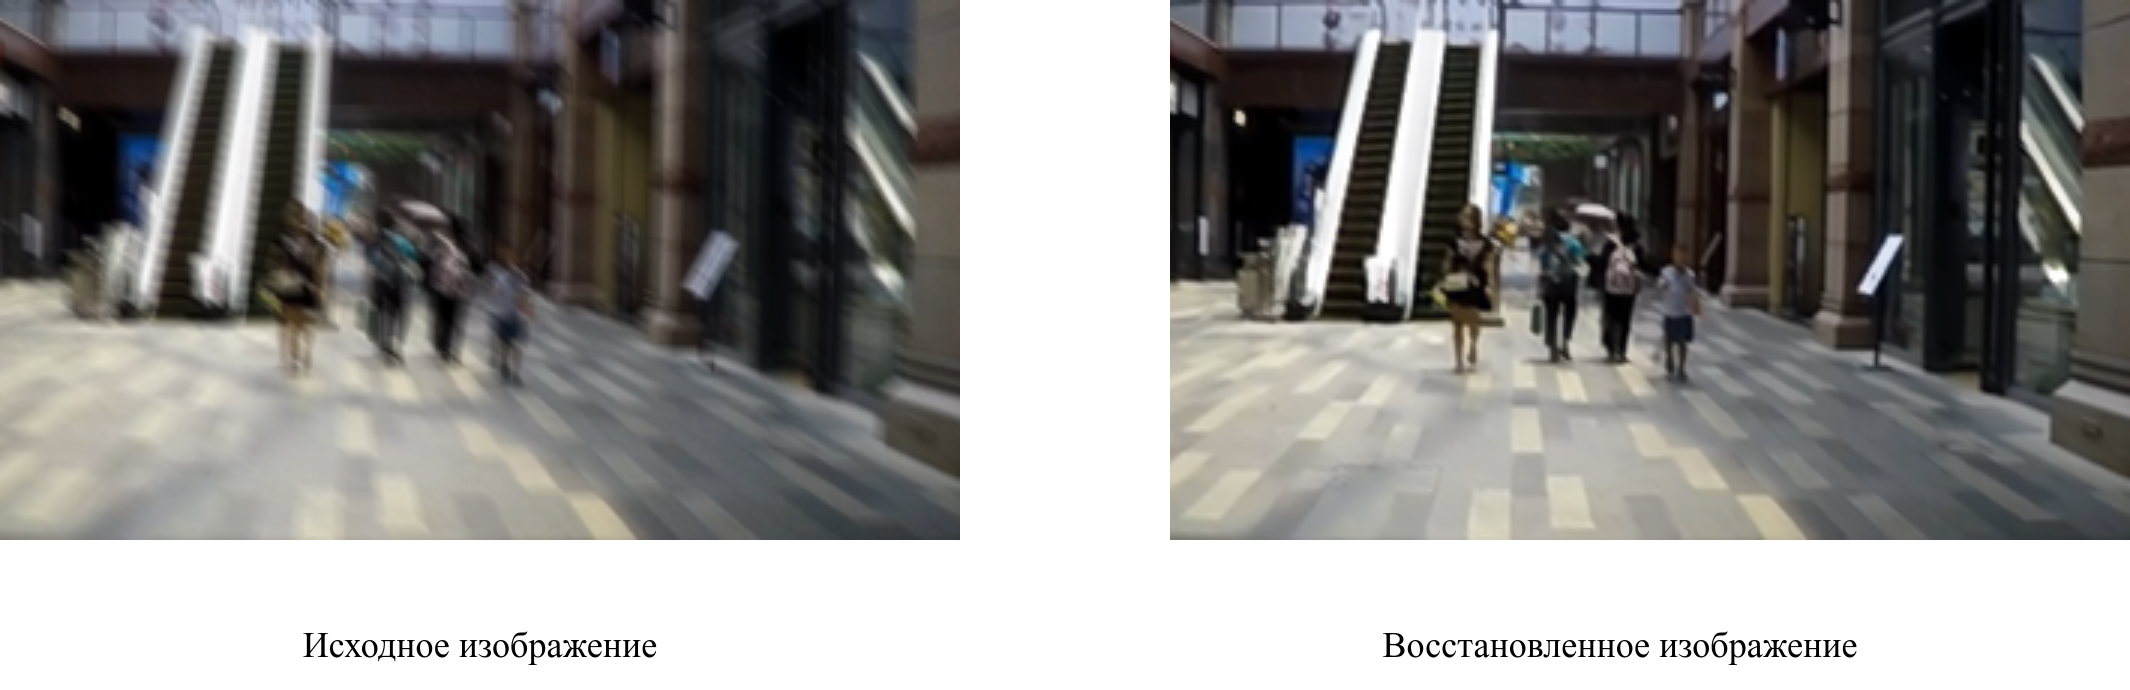
\includegraphics[width=1.0\textwidth]{assets/predict-result.png}
    \caption{Пример работы программы}
    \label{fig:demo}
\end{figure}

\section{Тестирование программное обеспечения}

Как было ранее указано, одним из требований MPRNet является то, что входное изображение должно быть одинаково разделено на четыре части. Поэтому в режиме оценки любое изображение, подаваемое на вход, дополняется нулевыми пикселями. После того как сеть выдает результат, эти дополненные пиксели удаляются, и предоставляется разрешение, которое было подано на вход сети. Кроме того, можно проводить тестирование сети следующим образом:

\begin{enumerate}[left=0.49cm]
    \item После нескольких эпох обучения сети можно приостановить обучение на обучающей выборке и проводить тестирование сети на списке изображений валидационной выборки. Таким образом, можно оценить работу метода на этапе обучения;
    \item С помощью обученных параметров весов можно проводить тестирование на некоторых парах изображений и оценить работу метода после прохождения этапа обучения. С использованием объективных метрик можно оценить работу метода после обучения;
    \item Пользователь может сам выбрать одно или несколько изображений и провести оценку работы метода относительно выбранных изображений.
\end{enumerate}
% исправляй грамматические ошибки и нормализируй текст если что убери слов и дополняй нормалных слов

\section*{Вывод}

В данном разделе проводилось описание выбранных средств реализации, аппаратных характеристик, процесса обучения нейросетевой модели и методов тестирования программного обеспечения.

Для реализации нейросетевой модели был выбран язык программирования Python, который обладает богатым набором библиотек для работы с нейросетями и обработки изображений, обучение нейросетевой модели проводилось на корпусе изображений GoPro, разрешение изображений было снижено для ускорения обучения.

Функция потерь модели включает в себя потерю Шарбонье и потерю края, которые оценивают разницу между предсказанными и исходными изображениями как по содержанию, так и по деталям.

Для тестирования программного обеспечения были разработаны методы, позволяющие оценить работу модели на различных этапах обучения, включая тестирование на валидационной выборке и отдельных изображениях.